\title{Loom: A new architecture for a high performance blockchain (WIP, v0.8.4) }

\author{
        Anatoly Yakovenko \\
        anatoly@loomprotocol.com\\
}
\date{}

\documentclass[12pt]{article}

% \usepackage{draftwatermark}
% \SetWatermarkText{Confidential}
% \SetWatermarkScale{5}
% \SetWatermarkColor[gray]{0.95}

\usepackage{graphicx}
\usepackage{bytefield}

\usepackage[]{hyperref}
\hypersetup{
    pdftitle={Loom: A new architecture for a high performance blockchain},
    pdfauthor={anatoly@loomprotocol.com},
    pdfsubject={blockchain},
    pdfkeywords={blockchain, bitcoin, cryptocurrency},
    bookmarksnumbered=true,     
    bookmarksopen=true,         
    bookmarksopenlevel=1,       
    colorlinks=true,            
    pdfstartview=Fit,           
    pdfpagemode=UseOutlines,    % this is the option you were lookin for
    pdfpagelayout=TwoPageRight
}

\begin{document}
\maketitle

\begin{abstract}
This paper proposes a Proof of History (PoH) - a proof for verifying passage of time between events. PoH is used to encode passage of time into a ledger - an append only data structure.  When used alongside a consensus algorithm such as Proof of Work (PoW) or Proof of Stake (PoS), PoH can reduce messaging overhead in a Byzantine Fault Tolerant replicated state machine.  This paper proposes two algorithms that leverage the time keeping properties of the PoH ledger - a Proof of Stake algorithm that can recover from partitions of any size and an efficient streaming Proof of Replication (PoRep).  The combination of PoRep and PoH provides a defense against forgery of the ledger with respect to time and storage.  The protocol is analyzed on a 1gbps network, and this paper shows that throughput up to 710k transactions per second is possible with today's hardware.
\end{abstract}

\section{Work In Progress}
This is a work in progress, for comments and suggestions please contact Anatoly Yakovenko anatoly@loomprotocol.com

\section{Introduction}
Blockchain is an implementation of a fault tolerant replicated state machine.  Current publicly available blockchains do not rely on time, or make a weak assumption about the participant's abilities to keep time~\cite{tendermint}.  Each node in the network usually relies on their own local clock without knowledge of any other participants clocks in the network.  The lack of a trusted source of time means that when a message timestamp is used to accept or reject a message, there is no guarantee that every other participant in the network will make the exact same choice.  The PoH presented here creates a ledger with verifiable passage of time, duration between events and message ordering. Every node in the network can rely on the recorded passage of time in the ledger without trust.

\section{Outline}
The remainder of this article is organized as follows. Overall system design is described in Section~\ref{design}. In depth description of Proof of History is described in Section~\ref{proof_of_history}. In depth description of the proposed Proof of Stake consensus algorithm is described in Section~\ref{proof_of_stake}. In depth description of the proposed fast Proof of Replication is described in Section~\ref{porep}. System Architecture and performance limits are analyzed in Section~\ref{system_architecture}. A high performance GPU friendly smart contracts engine is described in Section~\ref{sec:smartcontracts}

\section{Previous Work}\label{previous work}
TBD
\section{Design}\label{design}

\begin{figure}
  \begin{center}
    \centering
    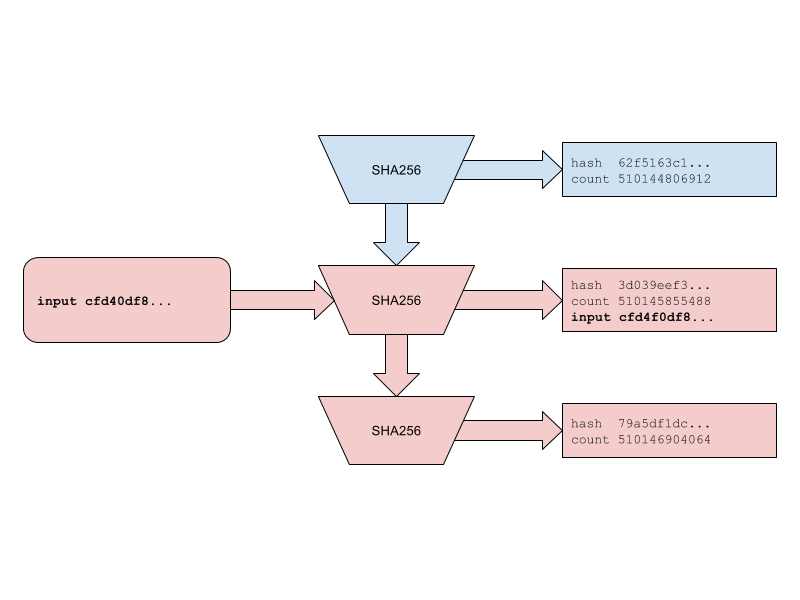
\includegraphics[width=0.8\textwidth]{figures/fig_1.png}
    \caption[Fig 1]{Transaction flow throughout the network.\label{fig:design}}
  \end{center}
  \end{figure}

As shown in Figure~\ref{fig:design}, Loom generates a Proof of History. It sequences user messages. It orders them such that they can be efficiently processed by maximizing throughput.  It executes the transactions on the current state that is stored in RAM. It publishes the transactions and a signature of the state to the replications nodes called Spools. Spools execute the same transactions on their copies of the state, and publish their computed signatures of the state as confirmations. The published confirmations serve as votes for the consensus algorithm.

There are many Looms in the network, and each Spool node has the same hardware capabilities as a Loom and can be elected as a Loom.  A Primary and lower ranked Looms are elected via a consensus algorithm. Elections for the proposed PoS algorithm are covered in depth in Section~\ref{subsec:elections}.

The Loom generates a Proof of History sequence, which along with global read consistency also provides a verifiable passage of time for the network.

In terms of CAP theorem, Consistency is almost always picked over Availability in an event of a Partition. In case of a large partition, this paper proposes a mechanism to eventually recover control of the network from a partition of any size.  This is covered in depth in Section~\ref{censorship}.

\section{Proof of History}\label{proof_of_history}

Proof of History provides a way to cryptographically verify passage of time between two events. It uses a cryptographically secure function whose output cannot be predicted from the input, and must be completely executed to generate the output. The function is run in a sequence, its previous output as the current input, periodically recording the current output, and how many times it's been called. The output can then be re-computed and verified by external computers in parallel by checking each period in parallel on a separate core. Data can be timestamped into this sequence by appending the data into the state of the function.  The recording of the state, index and data as it was appended into the sequences provides a timestamp that guarantees that the data was created sometime before the next hash was generated in the sequence. Horizontal scaling is also possible as multiple generators can synchronize amongst each other by mixing their state into each others sequences.  Horizontal scaling is discussed in depth in Section~\ref{poh:scale}\\

\subsection{Description}
With a cryptographic function, like a cryptographic hash (\texttt{sha256}, \texttt{md5}, \texttt{sha-1}), whose output cannot be predicted without running the function, run the function from some random starting value and take its output and pass it as the input into the same function again. Record the number of times the function has been called and the output at each call. The starting random value chosen could be any string, like the headline of the New York times for the day.
\\\\
\noindent For example: \\\\\noindent
\begin{center}
  \begin{tabular}{ | l | c | r |}
    \hline
    \multicolumn{3}{|c|}{PoH Sequence} \\
    \hline
    Index & Hash & Operation \\ \hline
    1 & hash1 & sha256(\char`\"any random starting value\char`\") \\ \hline
    2 & hash2 & sha256(hash1) \\ \hline
    3 & hash3 & sha256(hash2) \\ \hline
    \end{tabular}
\end{center}



\noindent Where \texttt{hashN} represents the actual hash output.\\

It is only necessary to publish a subset of the hashes and indices at an interval.\\

\noindent For example:\\\\\noindent
\begin{center}
  \begin{tabular}{ | l | c | r |}
    \hline
    \multicolumn{3}{|c|}{PoH Sequence} \\
    \hline
    Index & Hash & Operation \\ \hline
    1 & hash1 & sha256(\char`\"any random starting value\char`\") \\ \hline
    200 & hash200 & sha256(hash199) \\ \hline
    300 & hash300 & sha256(hash299) \\ \hline
    \end{tabular}
\end{center}


As long as the hash function chosen is collision resistant, this set of hashes can only be computed in sequence by a single computer thread, because there is no way to predict what the hash value at index $300$ is going to be without actually running the algorithm from the starting value $300$ times.  Thus we can infer from the data structure that time passed between index $0$ and index $300$.

\begin{figure}
  \begin{center}
    \centering
    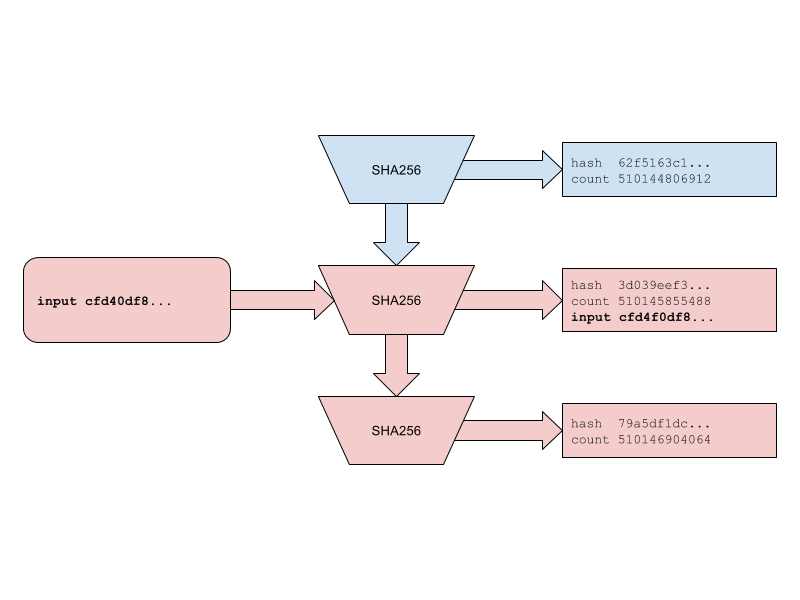
\includegraphics[width=0.6\textwidth]{figures/fig_2.png}
    \caption[Figure 2]{Proof of History sequence\label{fig:poh_seq}}
  \end{center}
  \end{figure}

In the example in Figure~\ref{fig:poh_seq}, hash \texttt{62f51643c1} was produced on
count $510144806912$ and hash \texttt{c43d862d88} was produced on
count $510146904064$. Real time passed between count $510144806912$
and count $510146904064$.

\subsection{Timestamp for Events}

This sequence of hashes can also be used to record that some piece of data was created before a particular hash index was generated. Using a `combine` function to combine the piece of data with the current hash at the current index. The `data` can simply be a cryptographically unique hash of arbitrary event data. The combine function can be a simple append of data, or any operation that is collision resistant. The next generated hash represents a "timestamp" of the data, because it could have only been generated after that specific piece of data was inserted.\\

\noindent For example:\\\\\noindent
\begin{center}
  \begin{tabular}{ | l | c | r |}
    \hline
    \multicolumn{3}{|c|}{PoH Sequence} \\
    \hline
    Index & Hash & Operation \\ \hline
    1 & hash1 & sha256(\char`\"any random starting value\char`\") \\ \hline
    200 & hash200 & sha256(hash199) \\ \hline
    300 & hash300 & sha256(hash299) \\ \hline
    \end{tabular}
\end{center}


\noindent Some external event occurs, like a photograph was taken, or
any arbitrary digital data was created:\\\\\noindent
\begin{center}
  \begin{tabular}{ | l | c | r |}
    \hline
    \multicolumn{3}{|c|}{PoH Sequence With Data} \\
    \hline
    Index & Hash & Operation \\ \hline
    1 & hash1 & sha256(\char`\"any random starting value\char`\") \\ \hline
    200 & hash200 & sha256(hash199) \\ \hline
    300 & hash300 & sha256(hash299) \\ \hline
    336 & hash336 & sha256(append(hash335, photograph\_sha256)) \\ \hline
    \end{tabular}
\end{center}


\texttt{Hash336} is computed from the appended binary data of
\texttt{hash335} and the \texttt{sha256} of the photograph. The index,
and the \texttt{sha256} of the photograph are recorded as part of the
sequence output. So anyone verifying this sequence can then recreate
this change to the sequence. The verifying can still be done in
parallel and its discussed in Section~\ref{poh:verify}

Because the initial process is still sequential, we can then tell that things entered into the sequence must have occurred sometime before the future hashed value was computed.\\\\\noindent

\begin{center}
  \begin{table}
  \begin{tabular}{ | l | c | r |}
    \hline
    Index & Hash & Operation \\ \hline
    1 & hash1 & sha256(\char`\"any random starting value\char`\") \\ \hline
    200 & hash200 & sha256(hash199) \\ \hline
    300 & hash300 & sha256(hash299) \\ \hline
    336 & hash336 & sha256(append(hash335, photograph1\_sha256)) \\ \hline
    400 & hash400 & sha256(hash399) \\ \hline
    500 & hash500 & sha256(hash499) \\ \hline
    600 & hash600 & sha256(append(hash599, photograph2\_sha256)) \\ \hline
    700 & hash700 & sha256(hash699) \\ \hline
    \end{tabular}
    \caption[Table 1]{PoH Sequence With 2 Events\label{table:multievent}}
    \end{table}
\end{center}

In the sequence represented by Table~\ref{table:multievent}, \texttt{photograph2} was created before \texttt{hash600}, and
\texttt{photograph1} was created before \texttt{hash336}. Inserting the data into the sequence of hashes results in a change to all subsequent values in the sequence. As long as the hash function used is collision resistant, and the data was appended, it is computationally impossible to pre-compute any future sequences based on prior knowledge of what data will be integrated into the sequence.\\

The data that is mixed into the sequence can be the raw data itself, or just a hash of the data with accompanying metadata.\\

\begin{figure}
  \begin{center}
    \centering
    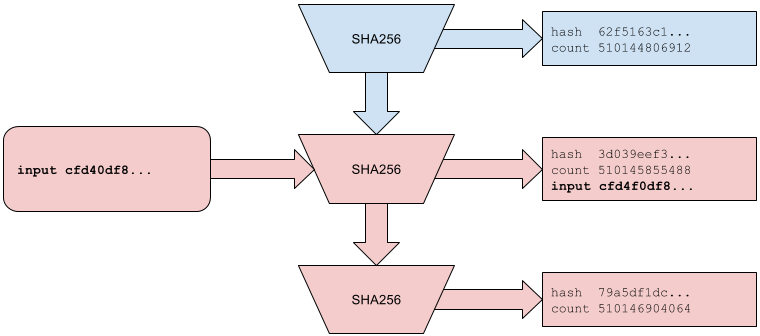
\includegraphics[width=0.6\textwidth]{figures/fig_3.png}
    \caption[Fig 3]{Figure description \label{fig:poh_insert}}
  \end{center}
  \end{figure}

  In the example in Figure~\ref{fig:poh_insert}, input \texttt{cfd40df8\ldots} was inserted into the Proof of History sequence. The count at which it was inserted is $510145855488$ and the state at which it was inserted it is \texttt{3d039eef3}.  All the future generated hashes are modified by this change to the sequence, this change is indicated by the color change in the figure.\\

Every node observing this sequence can determine the order at which all events have been inserted and estimate the real time between the insertions.

\subsection{Verification}\label{poh:verify}
The sequence can be verified as correct in a multi core computer in less time than it took to generated it \\

\noindent For example: \\\\\noindent
\begin{center}
  \begin{tabular}{ | l | c | r |}
    \hline
    \multicolumn{3}{|c|}{Core 1} \\
    \hline
    Index & Hash & Data \\ \hline
    200 & hash200 & sha256(hash199) \\ \hline
    300 & hash300 & sha256(hash299) \\ \hline
    \end{tabular}
  \begin{tabular}{ | l | c | r |}
    \hline
    \multicolumn{3}{|c|}{Core 2} \\
    \hline
    Index & Hash & Data \\ \hline
    300 & hash300 & sha256(hash299) \\ \hline
    400 & hash400 & sha256(hash399) \\ \hline
    \end{tabular}
\end{center}


So given some number of cores, like a modern GPU with $4000$ cores, the verifier can split up the sequence of hashes and their indexes into $4000$ slices, and in parallel make sure that each slice is correct from the starting hash to the last hash in the slice. So if the expected time to produce the sequence is going to be\\


\[
\frac{\textrm{Total number of hashes}}{\textrm{Hashes per second for 1 core}}
\]

\noindent The expected time to verify that the sequence is correct is going to be \\

\[
\frac{\textrm{Total number of hashes}}{\textrm{(Hashes per second per core * Number of cores available to verify)}}
\]

\begin{figure}
  \begin{center}
    \centering
    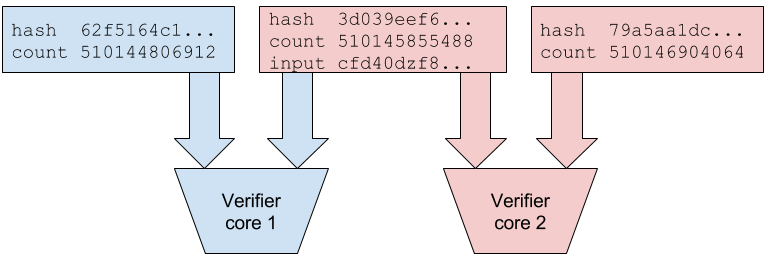
\includegraphics[width=0.6\textwidth]{figures/fig_4.png}
    \caption[Figure 4]{Verification using multiple cores\label{fig:poh_verify}}
  \end{center}
  \end{figure}

In the example in Figure~\ref{fig:poh_verify}, each core is able to verify each slice of the sequence in parallel. Since all input strings are recorded into the output, with the counter and state that they are appended to, the verifiers can replicate each slice in parallel.  The red colored hashes indicate that the sequence was modified by a data insertion.

\subsection{Horizontal Scaling}\label{poh:scale}
It's possible to synchronize multiple Proof of History generators by mixing the sequence state from each generator to each other generator, and thus achieve horizontal scaling of the Proof of History generator.  This scaling is done without sharding, the output of both generators is necessary to reconstruct the full order of events in the system.

\begin{center}
  \begin{tabular}{ | l | c | r |}
    \hline
    \multicolumn{3}{|c|}{PoH Generator A} \\
    \hline
    Index & Hash & Data \\ \hline
    1 & hash1a & \\ \hline
    2 & hash2a & hash1b \\ \hline
    3 & hash3a & \\ \hline
    4 & hash4a & \\
    \hline
    \end{tabular}
  \begin{tabular}{ | l | c | r |}
    \hline
    \multicolumn{3}{|c|}{PoH Generator B} \\
    \hline
    Index & Hash & Data \\ \hline
    1 & hash1b & \\ \hline
    2 & hash2b & hash1a \\ \hline
    3 & hash3b & \\ \hline
    4 & hash4b & \\
    \hline
    \end{tabular}
\end{center}

Given generators A and B, A receives a data packet from B (hash1b), which contains the last state from Generator B, and the last state generator B observed from Generator A. The next state hash in Generator A then depends on the state from Generator B, so we can derive that hash1b happened sometime before hash3a. This property can be transitive, so if three generators are synchronized through a single common generator \(A \leftrightarrow B \leftrightarrow C\), we can trace the dependency between A and C even though they were not synchronized directly.

By periodically synchronizing the generators, each generator can then handle a portion of external traffic, thus the overall system can handle a larger amount of events to track at the cost of true time accuracy due to network latencies between the generators.  A global order can still be achieved by picking some deterministic function to order any events that are within the synchronization window, such as by the value of the hash itself.


\begin{figure}
  \begin{center}
    \centering
    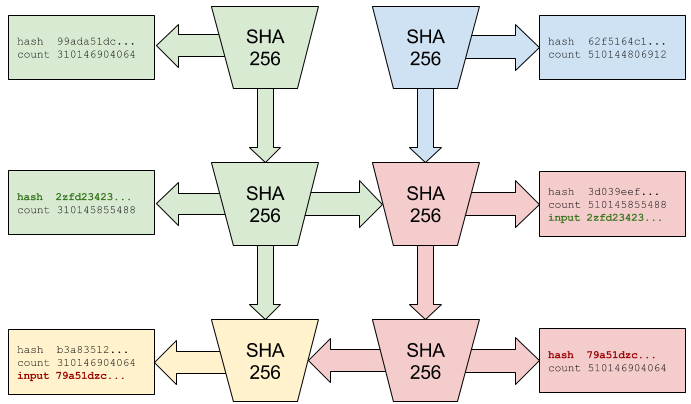
\includegraphics[width=0.6\textwidth]{figures/fig_5.png}
    \caption[Fig 5]{Two generators synchronizing\label{fig:poh_scale}}
  \end{center}
  \end{figure}

In Figure~\ref{fig:poh_scale}, the two generators insert each other’s output state and record the operation.  The color change indicates that data from the peer had modified the sequence.  The generated hashes that are mixed into each stream are highlighted in bold.

The synchronization is transitive. \(A \leftrightarrow B \leftrightarrow C\)  There is a provable order of events between A and C through B.

Scaling in this way comes at the cost of availability.  10x1gbps connections with availability of 0.999 would have \(0.999^{10} = 0.99 \) availability.

\subsection{Consistency}
Users can enforce consistency of the generated sequence and make it resistant to attacks by inserting the last observed output of the sequence they consider valid into their input.\\

\begin{center}
  \begin{tabular}{ | l | c | r |}
    \hline
    \multicolumn{3}{|c|}{PoH Sequence A} \\
    \hline
    Index & Hash & Data \\ \hline
    10 & hash10a & \\ \hline
    20 & hash20a & Event1 \\ \hline
    30 & hash30a & Event2 \\ \hline
    40 & hash40a & Event3 \\
    \hline
    \end{tabular}
  \begin{tabular}{ | l | c | r |}
    \hline
    \multicolumn{3}{|c|}{PoH Hidden Sequence B} \\
    \hline
    Index & Hash & Data \\ \hline
    10 & hash10a & \\ \hline
    20 & hash20a & Event3 \\ \hline
    30 & hash30a & Event2 \\ \hline
    40 & hash40a & Event1 \\
    \hline
    \end{tabular}
\end{center}

A malicious PoH generator could produce a second hidden sequence with the events in reverse order, if it has access to all the events at once, or is able to generate a faster hidden sequence.\\

To prevent this attack, each client generated Event should contain within itself the latest hash that the client observed from what it considers to be a valid sequence. So when a client creates the "Event1" data, they should append the last hash they have observed.\\

\begin{center}
  \begin{tabular}{ | l | c | r |}
    \hline
    \multicolumn{3}{|c|}{PoH Sequence A} \\
    \hline
    Index & Hash & Data \\ \hline
    10 & hash10a & \\ \hline
    20 & hash20a & Event1 = append(event1 data, hash10a) \\ \hline
    30 & hash30a & Event2 = append(event2 data, hash20a) \\ \hline
    40 & hash40a & Event3 = append(event3 data, hash30a) \\
    \hline
    \end{tabular}
\end{center}

When the sequence is published, Event3 would be referencing hash30a, and if it’s not in the sequence prior to this Event, the consumers of the sequence know that it’s an invalid sequence. The partial reordering attack would then be limited to the number of hashes produced while the client has observed an event and when the event was entered. Clients can then write software that does not assume the order is correct for the short period of hashes between the last observed and inserted hash.

To prevent a malicious PoH generator from rewriting the client Event hashes, the clients can submit a signature of the event data and the last observed hash instead of just the data.\\
\begin{center}
  \begin{tabular}{ | l | c | r |}
    \hline
    \multicolumn{3}{|c|}{PoH Sequence A} \\
    \hline
    Index & Hash & Data \\ \hline
    10 & hash10a & \\ \hline
    20 & hash20a & Event1 = sign(append(event1 data, hash10a), Client Private Key) \\ \hline
    30 & hash30a & Event2 = sign(append(event2 data, hash20a), Client Private Key) \\ \hline
    40 & hash40a & Event3 = sign(append(event3 data, hash30a), Client Private Key) \\
    \hline
    \end{tabular}
\end{center}

Verification of this data requires a signature verification, and a lookup of the hash in the sequence of hashes prior to this one.\\
\noindent Verify:\\\\\noindent
\texttt{
    (Signature, PublicKey, hash30a, event3 data) = Event3 \\
    Verify(Signature, PublicKey, Event3)\\
    Lookup(hash30a, PoHSequence)
}

\begin{figure}
  \begin{center}
    \centering
    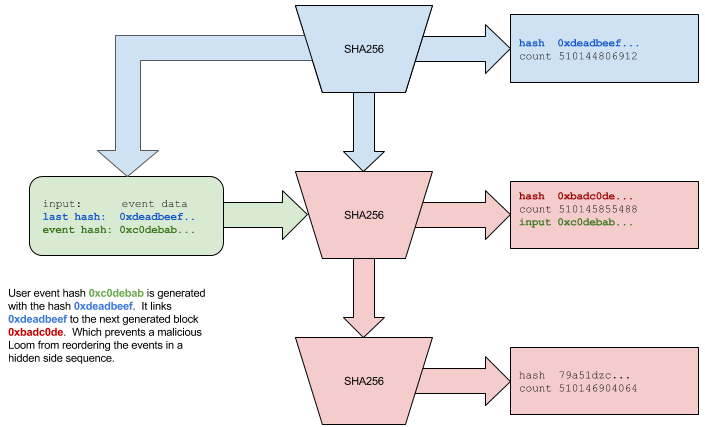
\includegraphics[width=0.6\textwidth]{figures/fig_6.png}
    \caption[Fig 6]{Input with a back reference.\label{fig:poh_consistency}}
  \end{center}
  \end{figure}

In Figure~\ref{fig:poh_consistency}, the user supplied input is dependent on hash 0xdeadbeef existing in the generated sequence sometime before it’s inserted.  The blue top left arrow indicates that the client is referencing a previously produced hash.  The clients message is only valid in a sequence that contains the hash 0xdeadbeef.  The red color in the sequence indicates that the sequence has been modified by the clients data.

\subsection{Overhead}
4000 hashes per second would generate an additional 160 kilobytes of data, and would require access to a GPU with 4000 cores and roughly 0.75-0.25 milliseconds of time to verify.

\subsection{Attacks}
\subsubsection{Reversal}
 Generating a reverse order would require an attacker to start the malicious sequence after the second event. This delay would allow any non malicious peer to peer nodes to communicate about the original order.

\subsubsection{Speed}
Having multiple generators may make deployment more resistant to attacks. One generator could be high bandwidth, and receive many events to mix into its sequence, another generator could be high speed low bandwidth that periodically mixes with the high bandwidth generator.

The high speed sequence would create a secondary sequence of data that an attacker would have to reverse.

\subsubsection{Long Range Attacks}

Long range attacks involve acquiring old discarded client Private Keys, and generating a falsified ledger~\cite{casper}.  Proof of history provides some protection against long range attacks. A malicious user that gains access to old private keys would have to recreate a historical record that takes as much time as the original one they are trying to forge. This would require access to a faster processor than the network is currently using, otherwise the attacker would never catch up in history length.

Additionally, a single source of time allows for construction of a simper Proof of Replication (more on that in Section~\ref{porep}). Since all the participants in the network can rely on a single historical record of events.

PoRep and PoH together provide a defense of both space and time against a forged ledger.


\section{Proof of Stake Consensus}\label{proof_of_stake}
\subsection{Description}
This specific instance of Proof of Stake is designed for quick confirmation of the current sequence produced by the Proof of History generator, for voting and selecting the next Proof of History generator, and for punishing any misbehaving validators. This algorithm depends on messages eventually arriving to all participating nodes within a certain timeout.
\subsection{Terminology}
\begin{description}

\item[bonds]
Bonds are equivalent to a capital expense in Proof of Work. A miner buys hardware and electricity, and commits it to a single branch in a Proof of Work blockchain. A bond is coin that the validator commits as collateral while they are validating transactions.

\item[slashing]

The solution to the nothing at stake problem in Proof of Stake systems~\cite{slasher}.  When a proof of voting for a different branch is published, that branch can destroy the validator's bond.  This is an economic incentive designed to discourage validators from confirming multiple branches.
\item[super majority]
A super majority is \(\frac{2}{3}\)rds of the validators weighted by their bonds.  A super majority vote indicates that the network has reached consensus, and at least \(\frac{1}{3}\)rd of the network would have had to vote maliciously for this branch to be invalid.  This puts the economic cost of an attack at \(\frac{1}{3}\)rd of the market cap of the coin.

\end{description}

\subsection{Bonding}
A bonding transaction takes a user specified amount of coin and moves it to a bonding account under the user’s identity. Coins in the bonding account cannot be spent, and have to remain in the account until the user removes them. The user can only remove stale coins that have timed out. Bonds are valid after super majority of the current stakeholders have confirmed the sequence.

\subsection{Voting}
Proof of History generator will publish a signature of the state at a predefined period. Each bonded identity must confirm that signature by publishing their own signed signature of the state. The vote is a simple Yes vote, without a no.

If super majority of the bonded identities have voted within a timeout, then this branch is accepted as valid.

\subsection{Unbonding}

Missing N number of votes marks the coins as stale and no longer eligible for voting. The user can issue an unbonding transaction to remove them.

N is a dynamic value based on the ratio of stale to active votes.  N increases as the number of stale votes increase.  In an event of a large network partition, this allows the larger branch to recover faster then the smaller branch.

\subsection{Elections}\label{subsec:elections}
Election for a new PoH generator occur when the PoH generator failure is detected. The validator with the largest voting power, or highest public key address if there is a tie is picked as the new PoH generator.

A super majority of confirmations are required on the new sequence. If the new leader fails before a super majority confirmations are available, the next highest validator is selected, and new set of conformations is required.

To switch votes, a validator needs to vote at a higher PoH sequence counter, and the new vote needs to contain the votes it wants to switch. Otherwise the second vote will be slashable. Vote switching can only occur at a height that does not have a super majority.

Once a PoH generator is established, a Secondary can be elected to take over the transactional processing duties. If a Secondary exists, it will be considered as the next leader during a Primary failure.

Secondary and lower rank generators are promoted to Primary at a predefined schedule, or if an exception is detected.
\subsection{Election Triggers}
\subsubsection{Forked Proof of History generator}

PoH generators have an identity that signs the generated sequence. A fork can only occur in case the PoH generator identity has been compromised. A fork is detected because two different historical records have been published on the same PoH identity.

\subsubsection{Runtime Exceptions}
A hardware failure or a bug, or a intentional error in the PoH generator could cause it to generate an invalid state and publish a signature of the state that does not match the local validators result. Validators will publish the correct signature via gossip and this event would trigger a new round of elections. Any validators who accept an invalid state will have their bonds slashed.

\subsubsection{Network Timeouts}

A network timeout would trigger an election.

\subsection{Slashing}
Slashing occurs when a validator votes two separate sequences. A proof of malicious vote will remove the bonded coins from circulation and add them to the mining pool.

A vote that includes a previous vote on a contending sequence is not eligible as proof of malicious voting. Instead of slashing the bonds, this vote removes remove the currently cast vote on the contending sequence.

Slashing also occurs if a vote is cast for an invalid hash generated by the PoH generator. The generator is expected to randomly generate an invalid state which would trigger a fallback to Secondary.
\subsection{Secondary Elections}
Secondary and lower ranked Proof of History generators can be proposed and approved. A proposal is cast on the primary generators sequence. The proposal contains a timeout, if the motion is approved by a super majority of the vote before the timeout, the Secondary is considered elected, and will take over duties as scheduled. Primary can do a soft handover to Secondary by inserting a message into the generated sequence indicating that a handover will occur, or inserting an invalid state and forcing the network to fallback to Secondary.

If a Secondary is elected, and the primary fails, the Secondary will be considered as the first fallback during an election.

\subsection{Attacks}
\subsubsection{Tragedy of Commons}

The PoS verifiers simply confirm the state hash generated by the PoH generator. There is economic incentive for them to do no work and simply approve every generated state hash. 

To avoid this condition, the PoH generator should generate an invalid hash with a probability P. Any voters for this hash should be slashed. When the hash is generated, the network should immediately promote the Secondary elected PoH generator.

\subsubsection{Collusion with the PoH generator}\label{subsubsec:collusion}
A verifier that is colluding with the PoH generator would know in advance when the invalid hash is going to be produced and not vote for it. This scenario is really no different than the PoH identity having a larger verifier stake. The PoH generator still has to do all the work to produce the state hash.
\subsubsection{Censorship}\label{censorship}
Censorship or denial of service could occur when \(\frac{1}{3}\)rd of the bond holders refuse to validate any sequences with new bonds. The protocol can defend against this form of attack by dynamically adjusting how fast bonds become stale. In the event of a denial of service, the larger partition can fork and censor the Byzantine bond holders. The larger network will recover as the Byzantine bonds become stale with time. The smaller Byzantine partition would not be able to move forward for a longer period of time. 

The algorithm would work as follows.  A majority of the network would elect a new Loom.  The Loom would then censor the Byzantine bond holders from participating.  Proof of History generator would have to continue generating a sequence, to prove the passage of time, until enough Byzantine bonds have become stale so the bigger network has a super majority.  The rate at which bonds become stale would be dynamically based on what percentage of bonds are active.  So the Byzantine minority fork of the network would have to wait much longer than the majority fork to recover a super majority.  Once a super majority has been established, slashing could be used to permanently punish the Byzantine bond holders.

\section{Streaming Proof of Replication}\label{porep}
\subsection{Description}
Filecoin proposed a version of Proof of Replication \cite{filecoinporep}. The goal of this version is to have fast and streaming verifications of Proof of Replication which are enabled by keeping track of time in Proof of History generated sequence. Replication is not used as a consensus algorithm, but is a useful tool to account for the cost of storing the blockchain history or state at a high availability.
\subsection{Algorithm}
As shown in Figure~\ref{fig:encrypt} CBC encryption encrypts each block of data in sequence, using the previously encrypted block to XOR the input data.

\begin{figure}
  \begin{center}
    \centering
    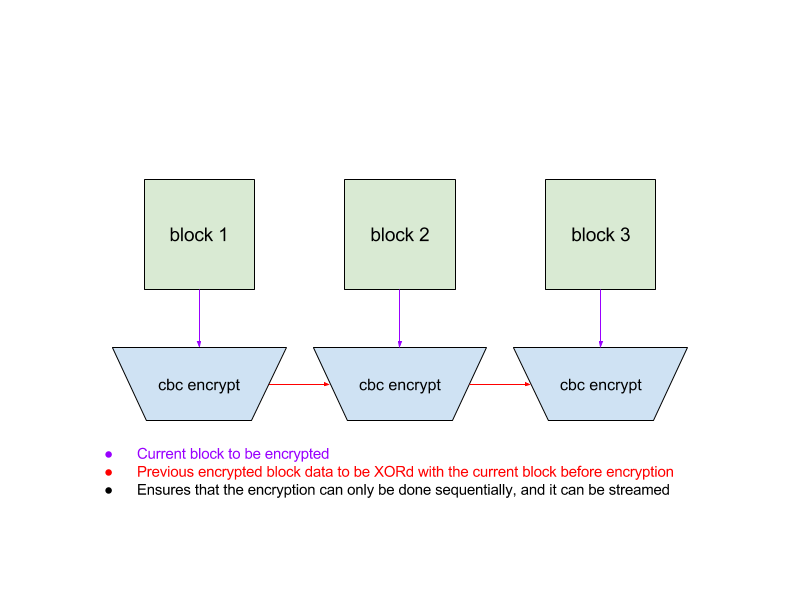
\includegraphics[width=0.6\textwidth]{figures/fig_7.png}
    \caption[Fig 7]{Sequential CBC encryption\label{fig:encrypt}}
  \end{center}
  \end{figure}

Each replication identity generates a key by signing a hash that has been generated Proof of History sequence. This ties the key to a replicators identity, and to a specific Proof of History sequence. Only specific hashes can be selected. (See Section~\ref{hashselection} on Hash Selection)

The data set is fully encrypted block by block. Then to generate a proof, the key is used to seed a pseudorandom number generator that selects a random 32 bytes from each block.

A merkle hash is computed with the selected PoH hash prepended to the each slice.

\begin{figure}
  \begin{center}
    \centering
    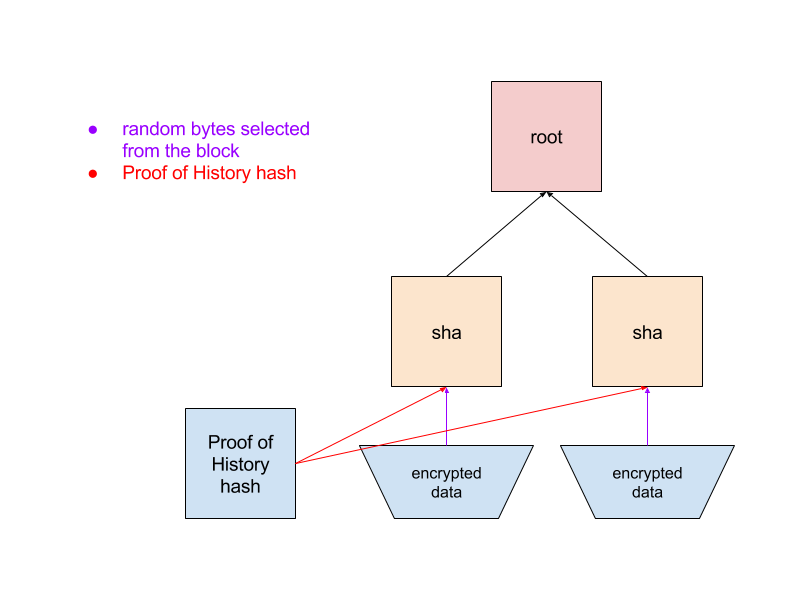
\includegraphics[width=0.6\textwidth]{figures/fig_8.png}
    \caption[Fig 8]{Fast Proof of Replication\label{fig_8}}
  \end{center}
  \end{figure}

The root is published, along with the key, and the selected hash that was generated. The replication node is required to publish another proof in N hashes as they are generated by Proof of History generator, where N is approximately \(\frac{1}{2}\) the time it takes to encrypt the data. The Proof of History generator will publish specific hashes for Proof of Replication at a predefined periods. The replicator node must select the next published hash for generating the proof. Again, the hash is signed, and random slices are selected from the blocks to create the merkle root.

After a period of N proofs, the data is re-encrypted with a new CBC key.
\subsection{Verification}

With N cores, each core can stream encryption for each identity. Total space required is \(2 blocks * N cores\), since the previous encrypted block is necessary to generate the next one. Each core can then be used to generate all the proofs that derived from the current encrypted block.

Total time to verify proofs is equal to the time it takes to encrypt. The proofs themselves consume few random bytes from the block, so the amount of data to hash is significantly lower then the encrypted block size.  The number of replication identities that can be verified at the same time is equal to the number of available cores. Modern GPUs have 3500+ cores available to them, albeit at \(\frac{1}{2}\)-\(\frac{1}{3}\)rd the clock speed of a CPU.

\subsection{Key Rotation}

Without key rotation the same encrypted replication can generate cheap proofs for multiple Proof of History sequences. Keys are rotated periodically and each replication is re-encrypted with a new key that is tied to a unique Proof of History sequence.

Rotation needs to be slow enough that it’s practical to verify replication proofs on GPU hardware, which is slower per core than CPUs.

\subsection{Hash Selection}\label{hashselection}

Proof of History generator publishes a hash to be used by the entire network for encrypting Proofs of Replication, and for using as the pseudorandom number generator for byte selection in fast proofs.

Hash is published at a periodic counter that is roughly equal to \(\frac{1}{2}\) the time it takes to encrypt the data set. Each replication identity must use the same hash, and use the signed result of the hash as the seed for byte selection, or the encryption key.

The period that each replicator must provide a proof must be smaller then the encryption time.  Otherwise the replicator can stream the encryption and delete it for each proof.

A malicious generator could inject data into the sequence prior to this hash to generate a specific hash. This attack is discussed more in \ref{subsubsec:collusion}.

\subsection{Proof Validation}
The Proof of History node does not validate the submitted Proof of Replication proofs. It only keep track of number of pending and verified proofs submitted by the replicators identity. A proof becomes verified when the replicator is able to sign the proof by a super majority of the validators in the network. 

The verifications are collected by the replicator via p2p gossip network, and submitted as one packet that contains a super majority of the validators in the network. This packet verifies all the proofs prior to a specific hash generated by the Proof of History sequence, and can contain multiple replicator identities at once.
\subsection{Attacks}
\subsubsection{Spam}
A malicious user could create many replicator identities and spam the network with bad proofs. To facilitate faster verification, nodes are required to provide the encrypted data and the entire merkle tree to the rest of the network when they request verification.

The Proof of Replication that is designed in this paper allows for cheap verification of any additional proofs, as they take no additional space. But each identity would consume 1 core of encryption time. The replication target should be set to a maximum size of readily available cores. Modern GPUs ship with 3500+ cores.

\subsubsection{Partial Erasure}

A replicator node could attempt to partially erase some of the data to avoid storing the entire state. The number of proofs, and the randomness of the seed should make this attack difficult.

For example, a user storing 1 terabyte of data erases a single byte from each 1 megabyte block.  A single proof that samples 1 byte out of every megabyte would have a likelihood of collision with any erased byte \(1 - (1- 1/1,000,0000)^{1,000,000} = 0.63\).  After 5 proofs the likelihood is \(0.99\).

\subsubsection{Collusion with PoH generator}

The signed hash is used to seed the sample. If a replicator could select a specific hash in advance then the replicator could erase all bytes that are not going to be sampled.

A replicator identity that is colluding with the proof of history generator could inject a specific transaction at the end of the sequence before the predefined hash for random byte selection is generated. With enough cores, an attacker could generate a hash that is preferable to the replicator identity.

This attack could only benefit a single replicator identity. Since all the identities have to use the same exact hash that is cryptographically signed with ECDSA (or equivalent), the resulting signature is unique for each replicator identity, and collision resistant. A single replicator identity would only have marginal gains.
\subsubsection{Denial of Service}
The cost of adding an additional replicator identity is equal to the cost of storage. The cost of adding extra computational capacity to verify all the replicator identities is equal to the cost of a CPU or GPU core per replication identity.

This creates an opportunity for a denial of service attack on the network by creating a large number of valid replicator identities.

To limit this attack, the consensus protocol chosen for the network can select a replication target, and award the replication proofs that meet the desired characteristics, like availability on the network, bandwidth, geolocation etc...
\subsubsection{Tragedy of Commons}

The PoS verifiers could simply confirm PoRep without doing any work. The economic incentives should be lined up with the PoS verifiers to do work, like by splitting the mining payout between the PoS verifiers and the PoRep replication nodes.

To further avoid this scenario, the PoRep verifiers can submit false proofs a small percentage of the time.  They can prove the proof is false by providing the function that generated the false data.  Any PoS verifier that confirmed a false proof would be slashed.

\section{System Architecture}\label{system_architecture}

\begin{figure}
  \begin{center}
    \centering
    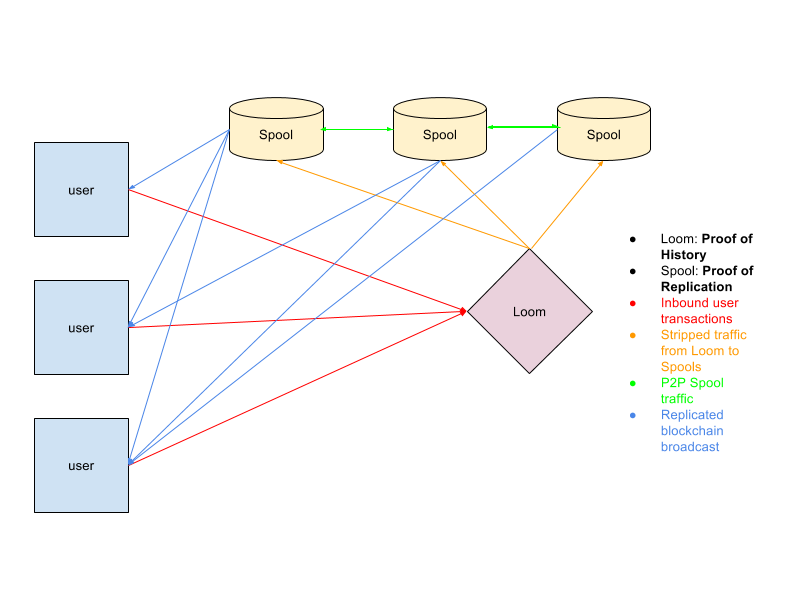
\includegraphics[width=0.6\textwidth]{figures/fig_9.png}
    \caption[Fig 9]{System Architecture \label{fig_9}}
  \end{center}
  \end{figure}

\subsection{Components}

\subsubsection{Loom, Proof of History generator}
The Loom is an elected Proof of History generator. It consumes arbitrary user transactions and outputs a Proof of History sequence of all the transactions that guarantees a unique global order in the system. After each batch of transactions the Loom outputs a signature of the state that is the result of running the transactions in that order. This signature is signed with the identity of the Loom.

\subsubsection{State}
A naive hash table indexed by the user’s address. Each cell contains the full users address and the memory required for this computation. For example\\
\noindent Transaction table contains:\\\\\noindent
\begin{bytefield}[bitwidth=.1em]{256}
\bitheader{0,31,63,95,127,159,191,223,255} \\
\bitbox{160}{Ripemd of Users Public Key}
& \bitbox{64}{Account}
& \bitbox{32}{unused}
\end{bytefield}\\
For a total of 32 bytes.\\
\noindent Proof of Stake bond’s table contains:\\\\\noindent
\begin{bytefield}[bitwidth=.1em]{256}
\bitheader{0,31,63,95,127,159,191,223,255} \\
\bitbox{160}{Ripemd of Users Public Key}
& \bitbox{64}{Bond} \\
& \bitbox{64}{Last Vote} \\
& \bitbox{224}{unused}
\end{bytefield}\\
For a total of 64 bytes.
\subsubsection{Spool, State Replication}
The Spool nodes replicate the blockchain state and provide high availability of the blockchain state. The replication target is selected by the consensus algorithm, and the validators in the consensus algorithm select and vote the Proof of Replication nodes they approve of based on of-chain defined criteria.

The network could be configured with a minimum Proof of Stake bond size, and a requirement for a single replicator identity per bond.
\subsubsection{Validators}
These nodes are consuming bandwidth from Spools. They are virtual nodes, and can run on the same machines as the Spools or the Loom, or on separate machines that are specific to the consensus algorithm configured for this network.

\subsection{Network Limits}

\begin{figure}
  \begin{center}
    \centering
    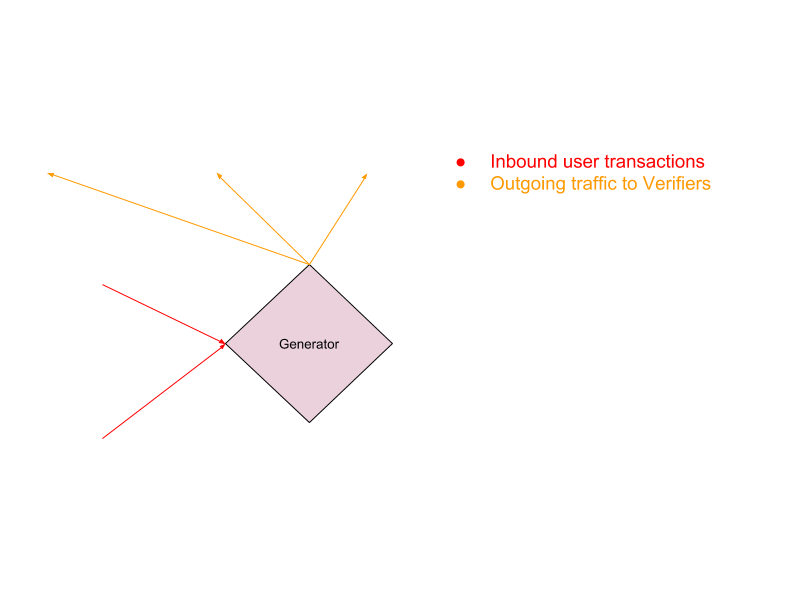
\includegraphics[width=0.8\textwidth]{figures/fig_10.png}
    \caption[Fig 10]{Loom network limits\label{fig_10}}
  \end{center}
  \end{figure}

Loom takes incoming user packets, orders them the most efficient way possible, and sequences them into a Proof of History sequence that is published to downstream Spools. Efficiency is based on memory access patterns of the transactions, so the transactions are ordered to minimize faults and to maximize prefetching.\\\\

\noindent Incoming packet format:\\\\\noindent
\begin{bytefield}[bitwidth=.1em]{256}
\bitheader{0,31,63,95,127,159,191,223,255} \\
\begin{rightwordgroup}{Signed}
\bitbox{160}{Last Valid Hash}
& \bitbox{64}{Counter}
& \bitbox{6}{u} 
& \bitbox{10}{s} \\
& \bitbox{64}{Fee} \\
& \bitbox{256}{From} \\
\end{rightwordgroup} \\
& \bitbox{256}{Signature 1/2} \\
& \bitbox{256}{Signature 2/2} \\
\end{bytefield}

\noindent Size \(20 + 8 + 16 + 8 + 32 + 32 32 = 148\) bytes.\\\\

The minimal payload that can be supported would be 1 destination account.
\noindent With Payload:\\\\\noindent
\begin{bytefield}[bitwidth=.1em]{256}
\bitheader{0,31,63,95,127,159,191,223,255} \\
\begin{rightwordgroup}{Signed}
\bitbox{160}{Last Valid Hash}
& \bitbox{64}{Counter}
& \bitbox{6}{u}
& \bitbox{10}{s} \\ 
& \bitbox{160}{To}
& \bitbox{64}{Amount} \\
& \bitbox{64}{Counter}
& \bitbox{64}{Fee} \\
& \bitbox{256}{From} \\
\end{rightwordgroup} \\
& \bitbox{256}{Signature 1/2} \\
& \bitbox{256}{Signature 2/2} \\
\end{bytefield}

\noindent With payload the minimum size: 176 bytes\\\\

The Proof of History sequence packet contains the current hash, counter, and the hash of all the new messages added to the PoH sequence and the state signature after processing all the messages.  This packet is sent once every N messages are broadcast.\\
\noindent Proof of History packet:\\\\\noindent
\begin{bytefield}[bitwidth=.1em]{256}
\bitheader{0,31,63,95,127,159,191,223,255} \\
\begin{rightwordgroup}{Signed}
\bitbox{160}{Current Hash}
& \bitbox{64}{Counter} \\
\bitbox{160}{Messages Hash} \\
\bitbox{160}{State Signature} \\
\end{rightwordgroup} \\
& \bitbox{256}{Signature 1/2} \\
& \bitbox{256}{Signature 2/2} \\
\end{bytefield}

\noindent Minimum size of the output packet is: 132 bytes \\\\

On a 1gbps network connection the maximum number of transactions possible is $1$~gigabit per second / $176$~bytes = $710$k tps max. Some loss $1-4\%$ is expected due to Ethernet framing. The spare capacity over the target amount for the network can be used to increase availability by coding the output with Reed-Solomon codes and striping it to the available downstream Spools.
\subsection{Computational Limits}
Each transaction requires a digest verification. This operation does not use any memory outside of the transaction message itself, and can be parallelized independent of all the other transactions. Thus throughput is going to be limited by the number of cores available on the system.

GPU based ECDSA verification servers have had experimental results of 900k operations per second~\cite{gpuecc}.
\subsection{Memory Limits}
A naive implementation of the state as a \(50\%\) full hashtable with 32 byte entries for each account, would fit 10 billion accounts into 640GB. Steady state random access to this table is measured at \(1.1 * 10^7\) writes or reads per second. Based on 2 reads and two writes per transaction, memory throughput can handle 2.75m transactions per second. This was measured on AWS 1TB x1.16xlarge instance.

\subsection{High Performance Smart Contracts}\label{sec:smartcontracts}

Smart contracts are a generalized form of transactions. These are programs that run on each node and modify the state. This design leverages extended Berkeley Packet Filter bytecode as fast and easy to analyze and JIT bytecode as the smart contracts language.

One of its main advantages is a zero cost Foreign Function Interface. Intrinsics, or high level functions that are implemented on the platform directly, are callable by user supplied programs. Calling the intrinsics suspends that program and schedules the intrinsic on a high performance server. Intrinsics are batched together to execute in parallel on the GPU.

\begin{figure}
  \begin{center}
    \centering
    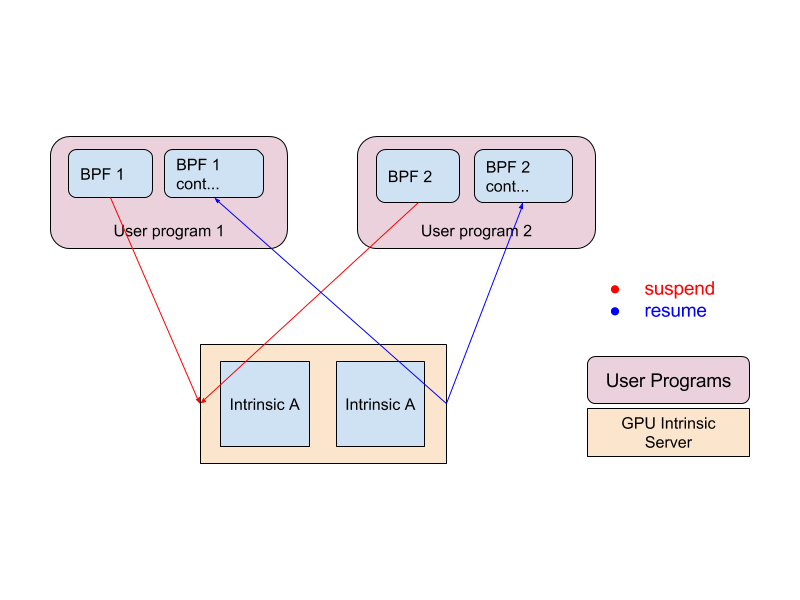
\includegraphics[width=0.6\textwidth]{figures/fig_11.png}
    \caption[Fig 11]{Executing user supplied BPF programs.\label{fig_11}}
  \end{center}
  \end{figure}

In the above example, two different user programs call the same intrinsic. Each program is suspended until the batch execution of the intrinsics is complete. An example common intrinsic is ECDSA verification. Batching these calls to execute on the GPU can increase throughput by thousands of times.

This trampoline requires no native Operating System thread context switches, since the BPF bytecode has a well defined context for all the memory that is using.

eBPF backend has been included in LLVM since 2015, so any LLVM frontend language can be used to write smart contracts. It’s been in the Linux kernel since 2015, and the first iterations of the bytecode have been around since 1992. A single pass can check eBPF for correctness, ascertain its runtime and memory requirements and convert it to x86 instructions.

\bibliographystyle{abbrv}
\bibliography{simple}

\begin{thebibliography}{9}
\bibitem{liskov}
Liskov, Practical use of Clocks
\\\texttt{ http://www.dainf.cefetpr.br/~tacla/SDII/PracticalUseOfClocks.pdf}

\bibitem{spanner}
Google Spanner TrueTime consistency
\\\texttt{ https://cloud.google.com/spanner/docs/true-time-external-consistency}

\bibitem{ordering}
Solving Agreement with Ordering Oracles
\\\texttt{ http://www.inf.usi.ch/faculty/pedone/Paper/2002/2002EDCCb.pdf}

\bibitem{tendermint}
Tendermint: Consensus without Mining
\\\texttt{https://tendermint.com/static/docs/tendermint.pdf}

\bibitem{filecoinporep}
Filecoin, proof of replication,
\\\texttt{https://filecoin.io/proof-of-replication.pdf}

\bibitem{slasher}
Slasher, A punative Proof of Stake algorithm
\\\texttt{https://blog.ethereum.org/2014/01/15/slasher-a-punitive-proof-of-stake-algorithm/}

\bibitem{delegatedpos}
BitShares Delegated Proof of Stake
\\\texttt{https://github.com/BitShares/bitshares/wiki/Delegated-Proof-of-Stake}

\bibitem{gpuecc}
An Efficient Elliptic Curve Cryptography Signature Server With GPU Acceleration
\\\texttt{http://ieeexplore.ieee.org/document/7555336/}

\bibitem{casper}
Casper the Friendly Finality Gadget
\\\texttt{https://arxiv.org/pdf/1710.09437.pdf}
\end{thebibliography}
\end{document}
This is never printed
